\documentclass[pdf, aspectratio=169]{beamer}
\usepackage[]{hyperref,graphicx,siunitx,lmodern,booktabs,tikz,pgfplots,marvosym,tensor}
\usepackage{pdfpc-commands}
\usepackage[mode=buildnew]{standalone}
\usepackage{cancel}
\mode<presentation>{\usetheme{Astro}}

\graphicspath{ {../Images/} }

\sisetup{per-mode=symbol}
\usetikzlibrary{calc,patterns, decorations.pathmorphing,shadings,fadings,intersections}

\pgfmathdeclarefunction{gauss}{3}{\pgfmathparse{#3*exp(-((x-#1)^2)/(2*#2^2))}}
\pgfdeclarehorizontalshading{rainbow}{100bp}{
  color(0bp)=(violet);
  color(30bp)=(black!30!violet); 
  color(38bp)=(blue);
  color(42bp)=(black!20!cyan);
  color(46bp)=(green); 
  color(52bp)=(yellow);
  color(58bp)=(orange);
  color(65bp)=(red); 
  color(73bp)=(black!60!red);
  color(100bp)=(black!50!red)
}

\newcommand{\linespectra}[2]{
  \coordinate (init) at (#1);
  \fill[shading=rainbow, opacity=0.1] (init) rectangle +(4,1);
  \draw[black,very thick] (init) rectangle +(4,1);
  \foreach \f in {#2}{
	\definecolor{col}{wave}{\f}
	%\fill[left color=transparent,right color=transparent,middle color=col] ($(init)+(\f/100-4,0)$) rectangle +(0.5mm,1cm);
	\fill[col, path fading=east] ($(init)+(\f/100-4+0.025,0)$) rectangle +(0.25mm,1cm);
	\fill[col, path fading=west] ($(init)+(\f/100-4+0.025,0)$) rectangle +(-0.25mm,1cm);
	%\node[white,anchor=west,font=\tiny, rotate=-90] at ($(init)+(\f/100-4+0.025,0)$) {\f nm};
  }
}

\newcommand{\absorbspectra}[2]{
  \coordinate (init) at (#1);
  \fill[shading=rainbow, opacity=0.8] (init) rectangle +(4,1);
  \draw[black,very thick] (init) rectangle +(4,1);
  \foreach \f in {#2}{
	\definecolor{col}{wave}{900}
	%\fill[left color=transparent,right color=transparent,middle color=col] ($(init)+(\f/100-4,0)$) rectangle +(0.5mm,1cm);
	\fill[col, path fading=east] ($(init)+(\f/100-4+0.025,0)$) rectangle +(0.25mm,1cm);
	\fill[col, path fading=west] ($(init)+(\f/100-4+0.025,0)$) rectangle +(-0.25mm,1cm);
	%\node[white,anchor=west,font=\tiny, rotate=-90] at ($(init)+(\f/100-4+0.025,0)$) {\f nm};
  }
}

%preamble
\title{Red vs Blue: Caboose goes fast}
\date{September 21, 2018}
\author{Jed Rembold}

\begin{document}
\renewcommand*{\theenumi}{\Alph{enumi}}

\begin{frame}{Announcements}
	\begin{itemize}
	  \item WebWorK due on Monday
	  \item Test a week from today!
		\begin{itemize}
		  \item What you'll need:
			\begin{itemize}
			  \item Pen/Pencil/Eraser
			  \item A basic calculator (It can't be your phone, sorry). If you don't have a friend to borrow from, I have about 6 that I can lend out, but you need to email me if you want one. First come, first served.
			  \item I'll try to limit how much actual calculator work is needed, but see previous test for an example
			\end{itemize}
		  \item Old tests and review questions posted
		  \item The same equation page as posted on the website will be included on the test
		  \item I'll write a test that takes me under 10 minutes to complete
		\end{itemize}
	  \item Polling: \nolinkurl{rembold-class.ddns.net}
	\end{itemize}
\end{frame}

\begin{frame}{The Sky \cancel{Tonight} Tomorrow!}
  \begin{itemize}
	\item Happy Fall Equinox tomorrow!
		\begin{itemize}
			\item Sun will rise directly in the East
			\item Will set directly in the West
			\item At the equator the Sun will be at zenith at noon
			\item Equal hours of day and night
		\end{itemize}
  \end{itemize}
\end{frame}

\begin{frame}{Review Question}
  What sort of object would you ascribe the below spectra to?
  \begin{center}
	
\begin{tikzpicture}[xscale=2.5]
	  \absorbspectra{0,0}{447,471,492,501,587,667}
	\end{tikzpicture}
  \end{center}
  \begin{enumerate}
	\item \alert<2>{A star with surrounding gases}
	\item A white hot chunk of nickel
	\item A helium lamp
	\item A diffuse gassy dinosaur
  \end{enumerate}
\end{frame}

\begin{frame}{The Remaining Light}
  We've two final issues to discuss with regards to light and spectra:
  \begin{itemize}
	\item<2-> Why don't stars (made of hydrogen) emit hydrogen lines?
	\item<3-> How can we tell if stars are moving?
  \end{itemize}
\end{frame}

\begin{frame}{Stars $\neq$ Gas Lamps}
  \begin{itemize}
	\item Atoms in close proximity to each other mess up each others energy levels
  \end{itemize}
	\begin{center}
		\begin{tikzpicture}
		  \only<1>{
			\fill[ball color=red] (0,0) circle (3pt);
			\foreach \r in {.5,1,...,2}{
			  \draw[yellow,dashed] (0,0) circle (\r cm);
			}
			\fill[ball color=cyan] (145:1) circle (2pt);
			\node at (270:2.5) {Lonely atom in thin gas};
			\draw[green,latex-] (2.4,0) -- +(1,0) node[align=center,right] {Nice, even\\energy levels};
		  }
		  \only<2>{
			\fill[ball color=red] (0,0) circle (3pt);
			\foreach \r in {.5,1,...,2}{
			  \draw[yellow,dashed] (-\r/2,0) circle (\r cm);
			}
			\fill[ball color=cyan] ($(145:1)-(.5,0)$) circle (2pt);
			\fill[ball color=red] (2.5,0) circle (3pt);
			\foreach \r in {.5,1,...,2}{
			  \draw[yellow,dashed] (2.5+\r/2,0) circle (\r cm);
			}
			\fill[ball color=cyan] ($(145:1)+(3,0)$) circle (2pt);
			\node at (1.25,-2.5) {Crowded atoms in dense gas};
			\node[green] (warp) at (1.25,2.5) {Warped energy levels!};
			\draw[-latex,green] (warp.south) --+(240:1);
			\draw[-latex,green] (warp.south)--+(300:1);
		  }
		\end{tikzpicture}
	  \end{center}
\end{frame}

\begin{frame}{Evolution of Spectra}
  \begin{center}
	\begin{tikzpicture}
	  \begin{axis}[samples=50, smooth,hide axis,width=10cm, height=6cm,xmin=-1]
		\only<1>{\addplot+[ultra thick, orange,mark=none,shading=rainbow] {gauss(0,.1,1)+gauss(2,.1,1.3)+gauss(4,.1,.8)}\closedcycle;}
		\only<2>{\addplot+[ultra thick, orange,mark=none,shading=rainbow] {gauss(0,.3,1)+gauss(2,.3,1.3)+gauss(4,.3,.8)}\closedcycle;}
		\only<3>{\addplot+[ultra thick, orange,mark=none,shading=rainbow] {gauss(0,.7,1)+gauss(2,.7,1.3)+gauss(4,.7,.8)}\closedcycle;}
		\only<4>{\addplot+[ultra thick, orange,mark=none,shading=rainbow] {gauss(0,1.3,1)+gauss(2,1.3,1.3)+gauss(4,1.3,.8)}\closedcycle;}
	  \end{axis}
	  \node<1> at (4,-1) {Low Density Gas};
	  \node<2> at (4,-1) {Higher Density Gas};
	  \node<3> at (4,-1) {Even Higher Density Gas};
	  \node<4> at (4,-1) {Really Dense Gas};
	\end{tikzpicture}
  \end{center}
\end{frame}

\begin{frame}{Time to Dopple}
  \begin{center}
	\inlineMovie{../Videos/Train_Horn.ogv}{../Videos/Train_Horn.jpg}{width=10cm}
  \end{center}
\end{frame}

\begin{frame}{The Doppler Effect}
  \begin{itemize}
	\item The Doppler effect affects \alert{all types} of waves, so this includes light!
	\item Approaching waves get compressed (smaller wavelengths)
	\item Receeding waves get stretched (larger wavelengths)
  \end{itemize}
  \begin{center}
	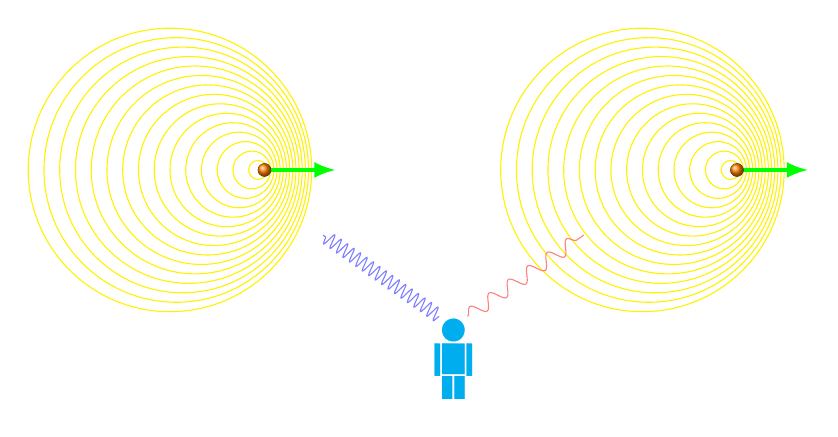
\begin{tikzpicture}[scale=.6]
	  \coordinate (s1) at (0,4);
	  \foreach \r in {.2,.4,...,3}{
		\draw[yellow] ($(s1)-(\r/1.5,0)$) circle (\r cm);
	  }
	  \draw[ultra thick, -latex,green] (s1) --+(1.5,0);
	  \fill[ball color=orange] (s1) circle (4pt);
	  \coordinate (s2) at (10,4);
	  \foreach \r in {.2,.4,...,3}{
		\draw[yellow] ($(s2)-(\r/1.5,0)$) circle (\r cm);
	  }
	  \draw[ultra thick, -latex,green] (s2) --+(1.5,0);
	  \fill[ball color=orange] (s2) circle (4pt);
	  
	  \node at (4,0) {\scalebox{4}{\textcolor{cyan}{\Gentsroom}}};
	  \draw[blue!50,decorate, decoration={snake,segment length=1mm}] (3.7,.9) --+(145:3);
	  \draw[red!50,decorate, decoration={snake,segment length=3mm,post length=0mm}] (4.3,.9) --+(35:3);
	\end{tikzpicture}
  \end{center}
\end{frame}

\begin{frame}{Putting Numbers to It}
  For our purposes:
  \[\frac{\lambda_{obs}-\lambda_{rest}}{\lambda_{rest}} = \frac{V}{c}\]
  Here:
  \begin{itemize}
	\item $\lambda_{obs}$ is the wavelength you see (observe)
	\item $\lambda_{rest}$ is the normal wavelength when not moving
	\item $V$ is the speed of the light source relative to you
	\item $c$ is the speed of light
  \end{itemize}
  \begin{block}{Careful, the sign of $V$ is important!}
	\begin{itemize}
	  \item a \textcolor{blue!50}{negative} $V$ means the source is coming toward you
	  \item a \textcolor{red!50}{positive} $V$ means the source is going away from you
	\end{itemize}
  \end{block}
\end{frame}

\begin{frame}{Applications to Astronomy}
  \begin{itemize}
	\item We can measure object speeds!
	\item Approaching objects are \alert{blueshifted}
	\item Receeding objects are \alert{redshifted}
  \end{itemize}
  \begin{center}
	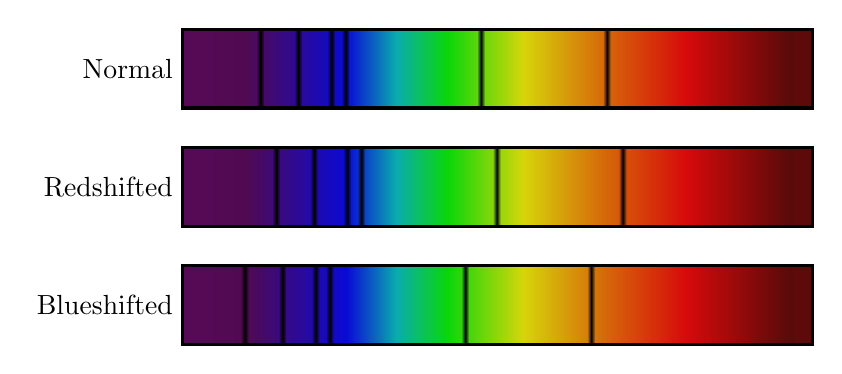
\begin{tikzpicture}[xscale=2]
	  \absorbspectra{0,0}{447,471,492,501,587,667}
	  \node[anchor=east] at (0,.5) {Normal};
	  \absorbspectra{0,-1.5}{457,481,502,511,597,677}
	  \node[anchor=east] at (0,-1) {Redshifted};
	  \absorbspectra{0,-3}{437,461,482,491,577,657}
	  \node[anchor=east] at (0,-2.5) {Blueshifted};
	\end{tikzpicture}
  \end{center}
\end{frame}

\begin{frame}{Example Time}
  \begin{example}
	As we'll talk about later, things near a black hole can get pretty crazy. Say a unfortunate friend (or maybe a dire enemy) is being sucked into a black hole and shining a \SI{550}{\nano\meter} green laser back at you. If they are traveling at a quarter the speed of light away from you, what wavelength do you perceive the laser to be at?
  \end{example}
\end{frame}

%\begin{frame}{Test Review}
  %\begin{itemize}
	%\item Specific questions?
	%\item Areas you want me to talk more on?
	%\item Questions about the test?
	%\item Concerns?
  %\end{itemize}
%\end{frame}

\begin{frame}{Telescope Time\ldots}
  \begin{center}
	\includegraphics[width=.7\textwidth]{ch16_telescope.jpg}
  \end{center}
\end{frame}

\begin{frame}{Looking at the Eye\ldots}
  \begin{columns}
	\column{.5\textwidth}
	\begin{itemize}
	  \item The Path of Light
		\begin{itemize}
		  \item Enters through pupil
		  \item Focused by lens
		  \item Projected onto retina
		\end{itemize}
	  \item Light entering at different angles gets focused in different locations
	  \item Your brain gets information on:
		\begin{itemize}
		  \item Wavelength (color)
		  \item Direction
		\end{itemize}
	\end{itemize}
	\column{.5\textwidth}
	\begin{center}
	  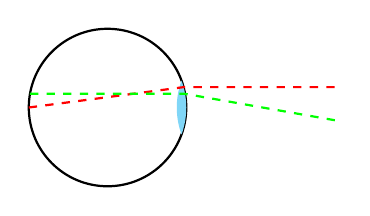
\begin{tikzpicture}
		\draw[thick] (0,0) circle (1cm);
		\fill[cyan!50] (-20:1) arc (-20:20:1) arc (160:200:1);
		\draw<2->[thick,red, dashed] (180:1) -- (15:1) --+ (2,0);
		\draw<3->[thick,green, dashed] (170:1) -- (10:1) --+ (-10:2);
	  \end{tikzpicture}
	\end{center}
  \end{columns}
\end{frame}

\begin{frame}{Cameras and Telescopes}
  \begin{itemize}
	\item Cameras are the simplest ``artificial'' eyes
	  \begin{itemize}
		\item Lenses still focus light
		\item Film takes the place of your retina
	  \end{itemize}
	\item Telescopes are essentially large cameras
	  \begin{itemize}
		\item May use a mirror to focus instead of a lens
		\item ``Retina'' can be film, photo-plates, or CCD detectors
	  \end{itemize}
  \end{itemize}
  \begin{center}
	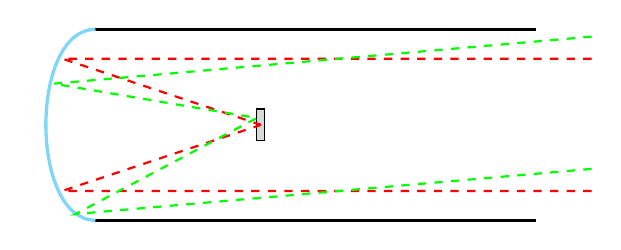
\begin{tikzpicture}[scale=1.4]
	  \draw[very thick] (60:1) --+(4,0);
	  \draw[very thick] (-60:1) --+(4,0);
	  \draw[very thick, cyan!50] (60:1) ..controls +(180:.6) and +(180:.6).. (-60:1);
	  \node[draw, minimum width=1mm, minimum height=4mm, inner sep=0pt, outer sep=0pt, fill=gray!30] (d) at (2,0) {};
	  \draw[red, dashed, thick] (5,.6) --+(-4.8,0) -- (d.center);
	  \draw[red, dashed, thick] (5,-.6) --+(-4.8,0) -- (d.center);
	  \draw[green, dashed, thick] (5,.8) --+(185:4.9) -- (d.120);
	  \draw[green, dashed, thick] (5,-.4) --+(185:4.7) -- (d.120);
	\end{tikzpicture}
  \end{center}
\end{frame}

\begin{frame}{Image Creation}
  \begin{itemize}
	\item To see a clear image:
	  \begin{itemize}
		\item Light coming from a single point on the object must go to a \emph{single point} on the image.
	  \end{itemize}
	\item Recall that light emits from a point on the object in all directions, so all of these must be properly redirected to a point on the image
  \end{itemize}
  \begin{center}
	\begin{tikzpicture}
	  \node[inner sep=0pt, outer sep=0pt] (obj) at (0,0) {\includegraphics[width=2cm]{tree.pdf}};
	  \fill[cyan!50] (4,-1) arc(-20:20:3) arc (160:200:3);
	  \node[inner sep=0pt, outer sep=0pt, xscale=-1, yscale=-1] (im) at (8,0) {\includegraphics[width=1cm]{tree.pdf}};
	  \foreach \y in {.8,.4,...,-1}{
		\draw[yellow, dashed] (obj.east) -- (4,\y) -- (im.east);
	  }
	  \draw[yellow, dashed, -latex, shorten >=-1cm] (obj.east) -- (4,1.2);
	  \draw[yellow, dashed, -latex, shorten >=-1cm] (obj.east) -- (4,-1.2);
	\end{tikzpicture}
  \end{center}
\end{frame}

\begin{frame}{Lenses and Mirrors}
  \begin{itemize}
	\item Lenses and mirrors redirect light to focus at a particular point
	\item Characterized by their \underline{focal point} or \underline{focal length}
	\item Parallel incoming light is redirected through the focal point
  \end{itemize}
  \begin{center}
	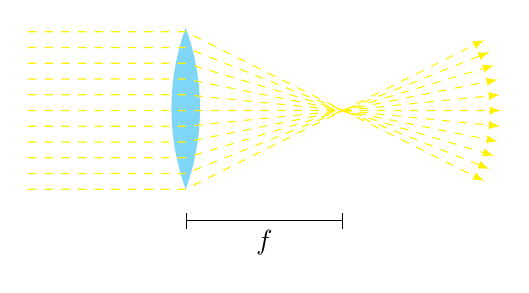
\begin{tikzpicture}
	  \coordinate (focus) at (2,0);
	  \coordinate (dummy) at (4,0);
	  \path (focus) -- (dummy); %To get centering correct
	  \fill[cyan!50] (0,-1) arc(-20:20:3) arc (160:200:3);
	  \foreach \y in {1,.8,...,-1}{
		\draw[yellow, dashed, shorten >=-2cm, -latex] (-2,\y) -- +(2,0) -- (focus);
	  }
	  \draw[|-|] (0,-1.4) -- (2,-1.4) node[midway, below] {$f$};
	\end{tikzpicture}
	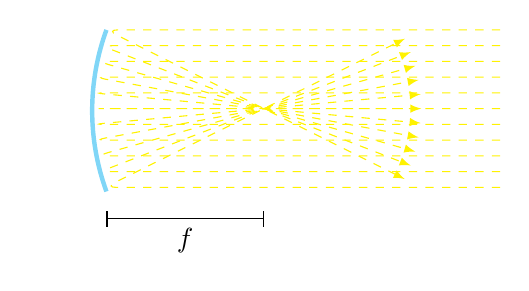
\begin{tikzpicture}
	  \coordinate (focus) at (2,0);
	  \coordinate (dummy) at (4,0);
	  \path (focus) -- (dummy); %To get centering correct
	  \draw[name path=lens, ultra thick,cyan!50] (0,1) arc (160:200:3);
	  \foreach \y in {1,.8,...,-1}{
		\path[name path=line] (5,\y) --+(-6,0);
		\draw[yellow, dashed, shorten >=-2cm, -latex, name intersections={of=line and lens, by=A}, rounded corners] (5,\y) -- (A) -- (focus);
	  }
	  \draw[|-|] (0,-1.4) -- (2,-1.4) node[midway, below] {$f$};
	\end{tikzpicture}
  \end{center}
\end{frame}

\begin{frame}{Ray Tracing}
  \begin{itemize}
	\item Two basic rules:
	  \begin{itemize}
		\item Rays that enter the lens/mirror parallel leave through the focus
		\item Rays that enter the lens/mirror through the focus leave parallel
	  \end{itemize}
	\item Recall the focal lengths exist on both sides of a lens!
  \end{itemize}
  \begin{center}
	\begin{tikzpicture}[scale=1.4]
	  \node[inner sep=0pt, outer sep=0pt] (obj) at (-3,0) {\includegraphics[width=2.0cm]{tree.pdf}};
	  \fill[cyan!50] (0,-1) arc(-20:20:3) arc (160:200:3);
	  \node[red] (f1) at (-1,0) {$\otimes$};
	  \node[red] (f2) at (1,0) {$\otimes$};
	  \draw[dashed, yellow, shorten >=-2cm] (obj.north) -- ($(0,1)!(obj.north)!(0,-1)$) -- (f2);
	  \draw[dashed, yellow, shorten >=-2cm] (obj.north) -- ($(obj.north)!3.2cm!(f1)$) --+(2,0);
	  \draw<2->[dashed, green, shorten >=-2cm] (obj.south) -- ($(0,1)!(obj.south)!(0,-1)$) -- (f2);
	  \draw<2->[dashed, green, shorten >=-2cm] (obj.south) -- ($(obj.south)!3.2cm!(f1)$) --+(2,0);
	  \node<3->[inner sep=0pt, outer sep=0pt, opacity=0.8, xscale=-1, yscale=-1] (obj) at (1.5,0) {\includegraphics[height=1cm]{tree.pdf}};
	\end{tikzpicture}
  \end{center}
\end{frame}

%\begin{frame}{Understanding Check}
  %The rocket below is being reflected in a curved mirror. How will its image compare to the rocket itself?
  %\begin{enumerate}
	%\item Flipped and Larger
	%\item \alert<3->{Flipped and Smaller}
	%\item Same orientation and Larger
	%\item Same orientation and Smaller
  %\end{enumerate}
  %\begin{center}
	%\begin{tikzpicture}[scale=1.4, transform shape]
	  %\node[inner sep=0pt, outer sep=0pt] (r) at (-5,0) {\includegraphics[width=2cm]{ch16_rocket.png}};
	  %\draw[ultra thick, cyan!50] (0,0) arc(0:20:4) (0,0) arc(0:-20:4);
	  %\node[red] (f) at (-1.5,0) {$\otimes$};

	  %\draw<2->[yellow, dashed, shorten >=-2cm] (r.north) --+(5,0) --(f);
	  %\draw<2->[yellow, dashed, shorten >=-2cm] (r.north) --($(r.north)!5.2cm!(f)$) --+(-2,0);
	  %\draw<2->[green, dashed, shorten >=-2cm] (r.south) --+(5,0) --(f);
	  %\draw<2->[green, dashed, shorten >=-2cm] (r.south) --($(r.south)!5.2cm!(f)$) --+(-2,0);
	  %\node<3->[inner sep=0pt, outer sep=0pt, xscale=-1, yscale=-1, opacity=0.7] at (-2.15,0) {\includegraphics[height=1cm]{ch16_rocket.png}};
	%\end{tikzpicture}
  %\end{center}
  %\end{frame}
\end{document}
